\chapter{\cernvmtestframework}
\subsection{Framework Design Overview}
\label{sct:frameworkoverview}

The \cernvmtestframework\ was initially designed to facilitate the role of ``Test Suites'' within the \releasetesting~infrastructure, which would 
execute tests and submit a report file in the form of a ``Test Anything Protocol'' (TAP) file to the ``Test Reports Framework''. This has since been
expanded to compensate for the shortcomings of \tapper and the \cernvmtestframework\ has since been expanded to comprise the role of the ``Test
Automation Framework'', which deploys, installs, and configures the \cernvm images before testing. This is important to understand as the 
``Precondition Tests'' shown in the following diagrams are mostly tests which facilitate the role of the ``Test Automation Framework'' by ensuring
that the \cernvm image host environment, and the images themselves are properly configured before executing the actual \cernvmreleasetesting test
cases.

\begin{figure}[!hbp]
	\begin{center}
		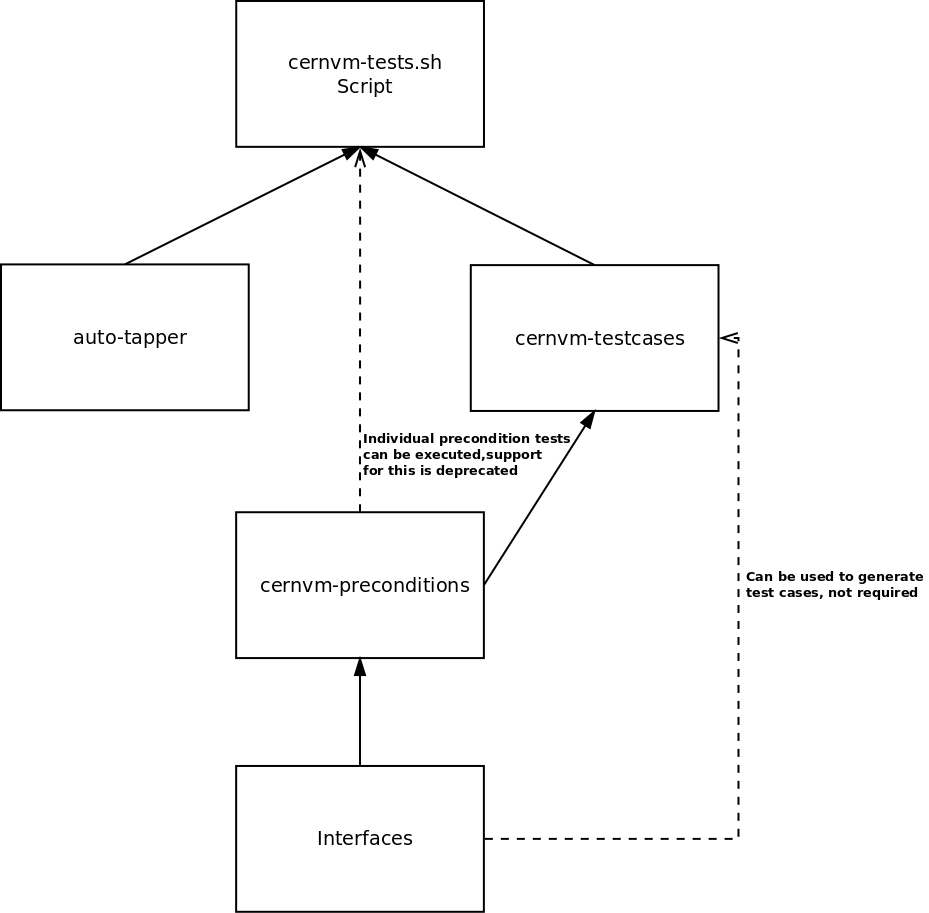
\includegraphics[scale=0.19]{img/proposed_framework.png}
	\end{center}
	\caption{Overview of the Proposed \cernvmtestframework}
	\label{fig:proposedarchitecture}
\end{figure}

\newpage
Currently, due to time constraints the optimal \cernvmtestframework\ design has not been implemented, figure~\ref{fig:proposedarchitecture} is a very
simplistic high-level overview of what the \emph{proposed} or intended final architecture is intended to be. The emphasis is on a hierarchical design
which is a result in part due to how scope is done in Bash and to limit the functions directly accessed by the {\bf cernvm-tests.sh} script to those
provided by auto-tapper and cernvm-testcases. In order for the proposed framework to be implemented, the \cernvm test cases must be modular test 
cases, independent of each other, this has not been implemented yet and as a result the following diagram outlines the current \cernvmtestframework.

\begin{figure}[hbp]
	\begin{center}
		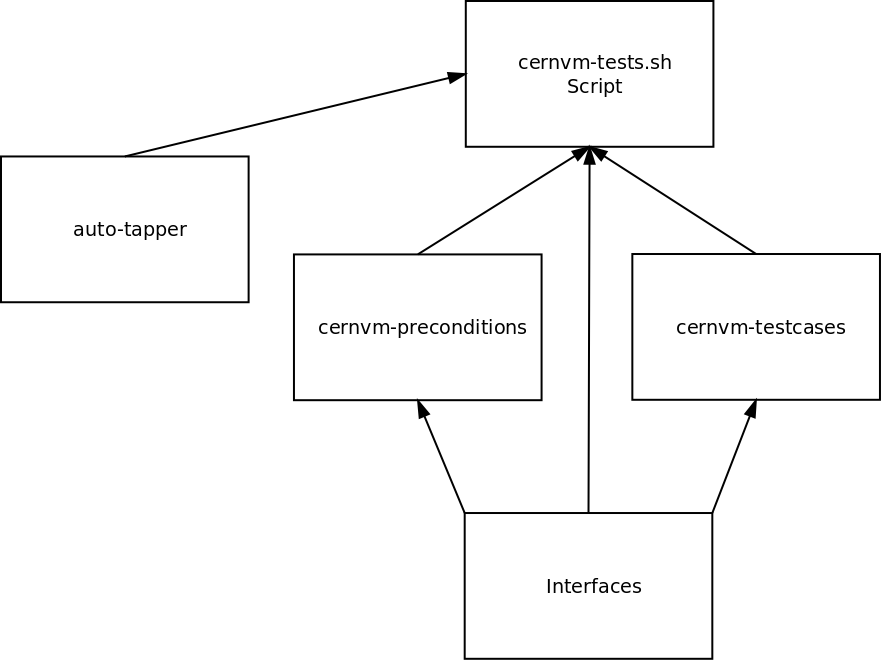
\includegraphics[scale=0.25]{img/current_framework.png}
	\end{center}
	\caption{Overview of the Current \cernvmtestframework}
	\label{fig:currentarchitecture}
\end{figure}

As shown in figure~\ref{fig:currentarchitecture} the current architecture of the \cernvmtestframework\ differs from the proposed framework because the
{\bf cernvm-tests.sh script}, \emph{which is the script that executes the set of \cernvm test cases}, requires both the {\bf cernvm-preconditions}
and {\bf cernvm-testcases} files. The {\bf cernvm-preconditions} file is what facilitates the ``Test Automation Framework'' by ensuring
that the host environment and \cernvm images are properly configured; the {\bf cernvm-testcases} file is what contains the actual
\cernvmreleasetesting test cases, which are required to test the \cernvm image. Inherently, this causes issues as there are precondition tests
that must pass before any of the test cases are executed for the results from the test cases to accurate. For example, in order to execute the test
case which verifies that the \cernvm image has SSH login support, numerous precondition tests must first be executed which create and configure the \cernvm image and verify that it can be started.

\begin{figure}[hbp]
	\begin{center}
		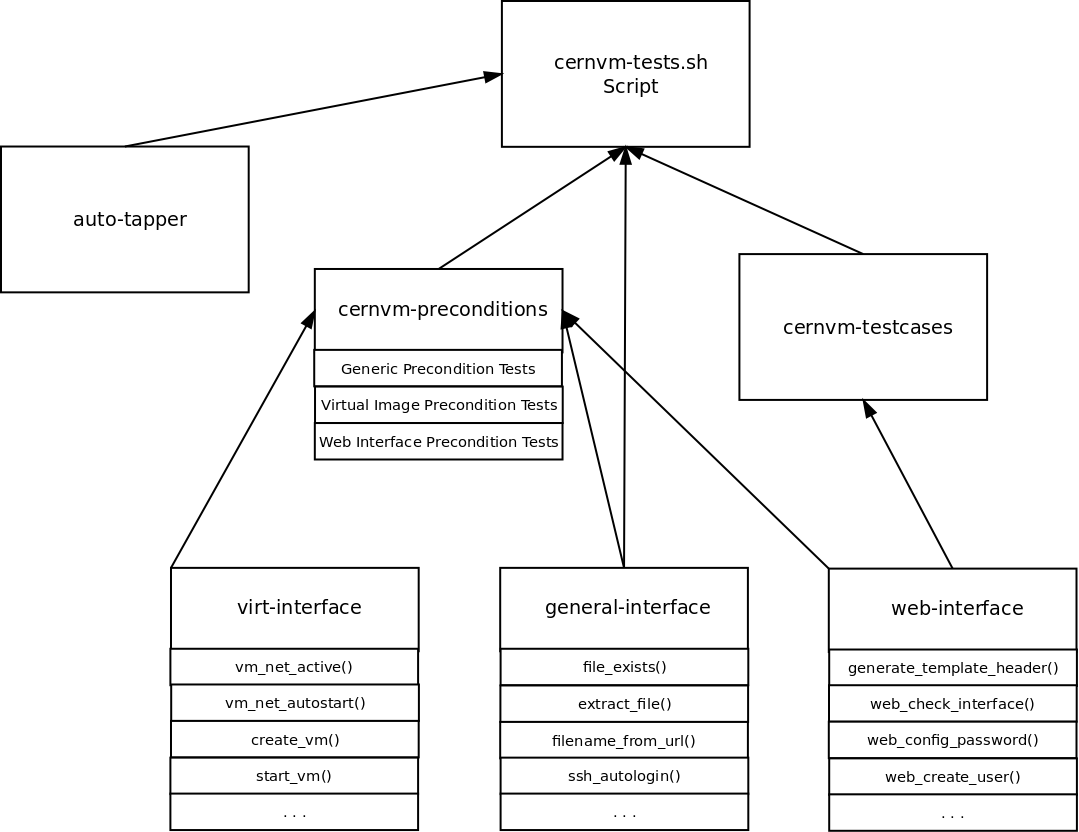
\includegraphics[scale=0.25]{img/detailed_framework.png}
	\end{center}
	\caption{Detailed Overview of the Current \cernvmtestframework}
	\label{fig:detailedarchitecture}
\end{figure}

The figure~\ref{fig:detailedarchitecture} provides a much more detailed diagram depicting the relations between the different files which are the
individual components that make up the current architecture of the \cernvmtestframework. As you can see, the hierarchy still exists to an extent
but because of the direct dependency the {\bf cernvm-tests.sh} script has on {\bf cernvm-preconditions} and {\bf cernvm-testcases} there are
precondition tests which must be executed first and in the correct order before any of the test cases can be executed.




\subsection{Precondition Tests}
\label{sct:preconditiontests}

Precondition tests are the tests which fulfil the role of the ``Test Automation Framework'' referred to in the \tapper architecture
figure~\ref{fig:architecture} within the \cernvmtestframework. The main purpose of the ``Precondition Tests'' is to ensure that the
host environment, and the \cernvm images themselves are properly configured before executing the actual \cernvmreleasetesting test
cases. The precondition tests configure the host environment and the \cernvm images through tests which automate deployment, 
installation, and configuration of the \cernvm images before testing.

Therefore, because the precondition tests are the tests which automate the process of setting up the host environment, the tests must
satisfied in order for a \cernvm test case to be executed accurately. In a nutshell, they are tests that must be executed, and pass before an 
actual test case can be executed. Currently, there are three categories of precondition tests, 

\begin{itemize}
\item	Generic Precondition Tests
\item	Virtual Image Precondition Tests
\item	Web Interface Precondition Tests
\end{itemize}

Generic precondition tests, as the name implies, are generic tests which provide functionality to configure the host environment and the
\cernvm image using methods that are not in the same category as the other two types of precondition tests. For example, a test that 
downloads and extracts the \cernvm image file, would be an example of a generic precondition test. Unlike generic precondition tests, 
virtual image precondition tests are very specific to configuring the virtualization environment of the \cernvm image and involve tests 
that interact with the libvirt/virsh library through the {\bf virt-interface} such as creating the virtual machine XML definition file 
and verifying the that the \cernvm image can be started. The last category of precondition tests, web interface precondition tests, 
are unique in that they are tests directly related to configuring the \cernvm image through the web interface of the \cernvm image. 
Although the web interface precondition tests could be expanded to include generic ``web'' tests, currently the precondition test are 
limited to configuring and controlling the \cernvm image through the web interface.




\subsection{\cernvm Test Cases}
\label{sct:cernvmtestcases}



- They are the tests which are used to make the cernvm test cases modular and
  independent of each other (ie. can execute boot errors test case before executing
  the web restart test case)
 